% !TEX root =main.tex

\section{El Concepte de 3BLD}

Per començar cal entendre el funcionament d'una resolució de blind, primer el cub és barrejat per una persona i el posa dins d'una capsa o un cube cover\footnote{Un cube cover és una tapa per cubs feta de cartró i que s'utlitza a les competicions}, després es col·loca a la taula boca avall i la persona que l'ha de resoldre es pren el seu temps per respirar.
Un cop fet això la persona que resol el cub encén el timer i destapa el cub, de manera que el temps comença a comptar i es comença a memoritzar. Un cop acabada la memorització el que resol el cub es tapa els ulls amb un antifaç i comença a resoldre el cub, mentre que una persona externa li posa una cartiluna entre el cub i la seva cara per evitar trampes i mirar per sota de l'antifaç.
Tots aquests passos s'han d'executar perfectament per asegurar-se de la resolució compti.

\begin{figure}[ht]
    \centering
    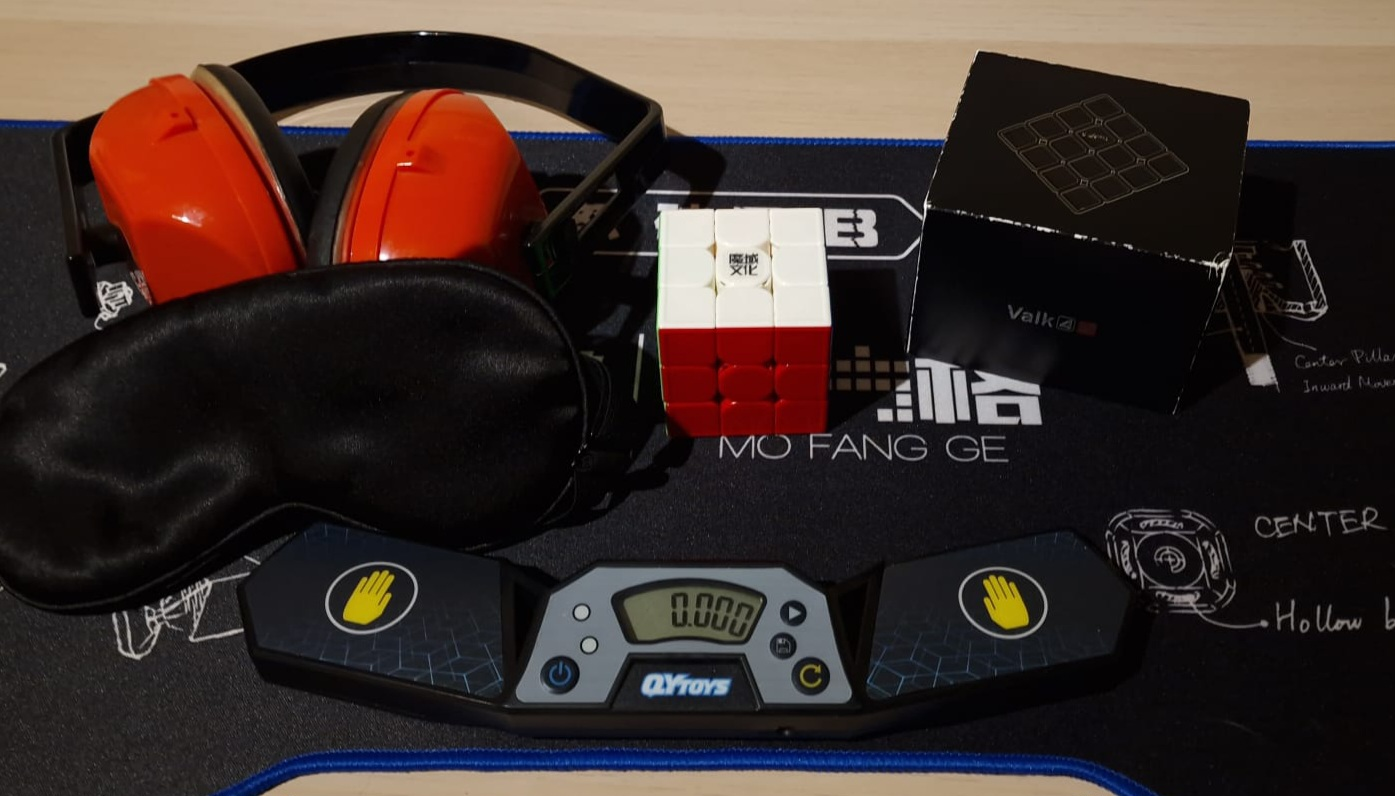
\includegraphics[width=12cm]{img/figures/materials-bld.jpg}
    \caption{Materials necessaris per poder executar blind}
    \label{fig:materials-bld}
\end{figure}


\vspace{0.5cm}
\subsection{Fases de la Resolució}

Com ja he esmentat a la seccio anterior, completar el cub de Rubik amb els ulls tancats, es divideix en dos grans fases, memorització i execució. I dins d'aquestes fases hi han diferents procediments per poder aconseguir fer-ho correctament.

\subsection{Memorització}


En aquesta fase com ja ho diu el seu nom has de memoritzar el cub. La manera de memoritzar no és la més convencional ja que no memoritzes color sinó peces i com que hem d'interpretar el cub  com si fossin 20 peces el que fem es donar-li una lletra per la qual pots identificar a cada peça. Fent aquestes conversions has d'arribar a tenir el teu propi esquema de lletres, el que utilitzo jo és el de la figura \ref{fig:letter-scheme}, i el pots agafar com a plantilla per fer el teu o directament utilitzar-lo ja que si t'acostumes no et limitarà res durant el procés.

\begin{figure}[ht]
    \centering
    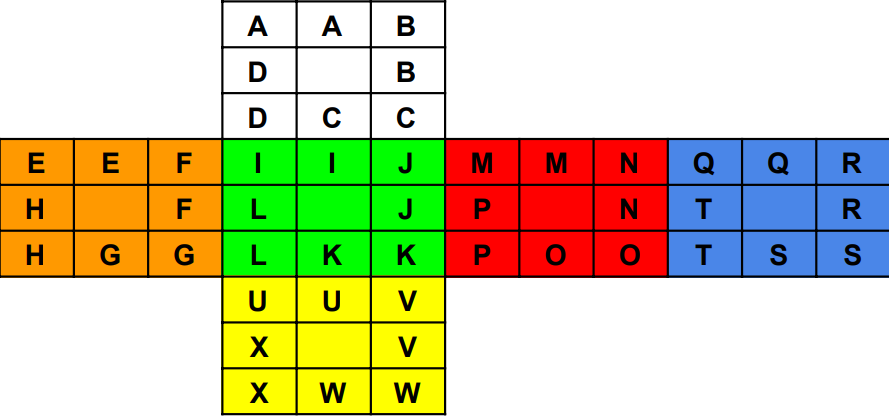
\includegraphics[width=12cm]{img/figures/letter-scheme.png}
    \caption{Esquema de Lletres}
    \label{fig:letter-scheme}
\end{figure}

Hi han lletres repetides perquè primer memoritzes arestes i després cantonades, aquestes lletres a l'hora de memoritzar-les, no les memoritzes a força bruta, sinó que les converteixes en paraules que puguis convertir en imatges per poder entrecordar-te. Sembla molt complex però no ho és com es pot veure en el següent exemple.
Per practicar aquesta transformació d'imatges pots anar a la pàgina web \href{https://polsances13.github.io/roadto3bld/App.Html}{roadto3bld} on podràs veure el codi de la app i on hi haurà un link a github on podràs descarregar i utilitzar l'app.
\vspace{0.25cm}

$$ \textrm{Haig de memoritzar les lletres R i B    }  \rightarrow \textrm{   RedBull} $$
$$ \textrm{Haig de memoritzar les lletres A i C   }  \rightarrow \textrm{   Aire Acondicionat (AC és el símbol)} $$

Llavors has de tenir per a cada parell de lletres una paraula clau per memoritzarles ràpidament. Et pots inspirar en les d'algú, com les meves de les taules al final del document, però aquestes si que no les hauries de copiar, ja que aquestes paraules han de ser les que primer et vinguin al cap pensant en les dues lletres, és un treball una mica pesat però amb el temps dona el seu fruit.
No hi ha secret per integrar aquestes paraules a la teva ment, el que has de fer és practicar, practicar i practicar, i amb el temps et sortirà sol.

\begin{table}[ht]
    \centering
    \begin{tabular}{|l|l|l|l|}
        \hline
        AA & AA                 & BL & BL                      \\ \hline
        AB & ABS                & BM & BM (spam)               \\ \hline
        AC & Aire Acondicionat  & BN & BiNari                  \\ \hline
        AD & AD (Anunci)        & BO & BOB                     \\ \hline
        AE & Aero               & BP & BP (gasolinera)         \\ \hline
        AF & AFRO               & BQ & BQ (marca de mòbils)    \\ \hline
        AG & AG (PLATA)         & BR & BRR (so)                \\ \hline
        AH & AHORA              & BS & BS (abreviació de text) \\ \hline
        AI & AI (Onomatopeia)   & BT & BlueTooth               \\ \hline
        AJ & AJO                & BU & BU (so)                 \\ \hline
        AK & AK-47              & BV & BBVA                    \\ \hline
        AL & ALUMINI            & BW & BBW (brake by wire)     \\ \hline
        AM & AM                 & BX & BoX                     \\ \hline
        AN & AN                 & CA & Catalunya               \\ \hline
        AO & AVERAGE OF         & CB & CB (defensa central)    \\ \hline
        AP & APP                & CC & CC (correu)             \\ \hline
        AQ & AQuaman            & CD & CD                      \\ \hline
        AR & AR SPEEDCUBER      & CE & CEo                     \\ \hline
        AS & AS                 & CF & CoFre                   \\ \hline
        AT & AlphaTauri         & CG & Centre de Gravetat      \\ \hline
        AU & AU (Onomatopeia)   & CH & CHili                   \\ \hline
        AV & AVE                & CI & CI (compl indirecte)    \\ \hline
        AW & AWard              & CJ & CJ                      \\ \hline
        AX & AXE                & CK & CooK                    \\ \hline
        BA & BALA               & CL & ClocK                   \\ \hline
        BB & BEBÉ               & CM & Càmera                  \\ \hline
        BC & BC (Before Christ) & CN & CN (compl nom)          \\ \hline
        BD & BuD                & CO & CO (companyia)          \\ \hline
        BE & Bed                & CP & Codi Postal             \\ \hline
        BF & BFF                & CQ & CaQui                   \\ \hline
        BG & BackGround         & CR & CR (continental record) \\ \hline
        BH & BH (BICICLETES)    & CS & CS (computer science)   \\ \hline
        BI & BI                 & CT & CTT                     \\ \hline
        BJ & BeiJing            & CU & CUb                     \\ \hline
        BK & BreaK              & CV & CV (curric.vitae)       \\ \hline
    \end{tabular}
    \caption{Taula de Parells de Lletres AA \rightarrow CV}
    \label{tla:lletres-1}
\end{table}

\begin{table}[ht]
    \centering
    \begin{tabular}{|l|l|l|l|}
        \hline
        CW & CoW               & EJ & EJect                 \\ \hline
        CX & CX (Citroen)      & EK & EKA (mètode)          \\ \hline
        DA & DA (sí en Rus)    & EL & EL                    \\ \hline
        DB & DataBase          & EM & Eminem                \\ \hline
        DC & DC (Distr of C)   & EN & EN                    \\ \hline
        DD & DoDo              & EO & EO (edge orientation) \\ \hline
        DE & DE                & EP & EP                    \\ \hline
        DF & Districte Federal & EQ & EquiP                 \\ \hline
        DG & DoG               & ER & ER (European record)  \\ \hline
        DH & DHl               & ES & Espanya               \\ \hline
        DI & DIA               & ET & ET                    \\ \hline
        DJ & DJ                & EU & Estats Units          \\ \hline
        DK & Donkey Kong       & EV & EVO                   \\ \hline
        DL & DòLar             & EW & EW (so)               \\ \hline
        DM & DuMb              & EX & EX                    \\ \hline
        DN & DaN               & FA & Fa (nota musical)     \\ \hline
        DO & DO (nota musical) & FB & FaceBook              \\ \hline
        DP & DP (empresa)      & FC & FC (futbol club)      \\ \hline
        DQ & DsQ               & FD & Feed                  \\ \hline
        DR & Domino Reduction  & FE & FE                    \\ \hline
        DS & DS (Nintendo)     & FF & ForceFeedback         \\ \hline
        DT & DoT               & FG & FueGo                 \\ \hline
        DU & DUo               & FH & FarenHeit             \\ \hline
        DV & DaVid             & FI & FInlandia             \\ \hline
        DW & DeU               & FJ & FiJi                  \\ \hline
        DX & DuX               & FK & FaKe                  \\ \hline
        EA & EA (empresa)      & FL & FLuid                 \\ \hline
        EB & EB (Buggati)      & FM & FM (radio)            \\ \hline
        EC & ECo               & FN & FortNite              \\ \hline
        ED & Educació          & FO & FOca                  \\ \hline
        EE & EE (so)           & FP & FP                    \\ \hline
        EF & EFecte            & FQ & FaQ                   \\ \hline
        EG & EG (mètode)       & FR & FRança                \\ \hline
        EH & EH (so)           & FS & For Speed             \\ \hline
        EI & Einstein          & FT & Foto                  \\ \hline
    \end{tabular}
    \caption{Taula de Parells de Lletres CW \rightarrow FT}
    \label{tla:lletres-2}
\end{table}


\begin{table}[ht]
    \centering
    \begin{tabular}{|l|l|l|l|}
        FU & FUm            & HH & Hula Hop             \\\hline
        FV & FiVerr         & HI & HIppie               \\\hline
        FW & ForWard        & HJ & HiJo                 \\\hline
        FX & FaX            & HK & Honk Kong            \\\hline
        GA & GA (perm)      & HL & HaLo                 \\\hline
        GB & GB (perm)      & HM & HuM                  \\\hline
        GC & GC (perm)      & HN & HaN                  \\\hline
        GD & GoD            & HO & Ho Ho                \\\hline
        GE & GEl            & HP & HP (marca)           \\\hline
        GF & GiF            & HQ & High Quality         \\\hline
        GG & GG             & HR & Heart Rate           \\\hline
        GH & GraHam         & HS & High School          \\\hline
        GI & GIrona         & HT & HoT                  \\\hline
        GJ & Good Job       & HU & HUngary              \\\hline
        GK & GoKu           & HV & HaVe                 \\\hline
        GL & GL             & HW & HomeWork             \\\hline
        GM & Grand Master   & HX & HeXA                 \\\hline
        GN & GaN            & IA & IA (chatgpt)         \\\hline
        GO & GO             & IB & IBai                 \\\hline
        GP & Gran Premi     & IC & ICono                \\\hline
        GQ & GRAN QUESO     & ID & ID                   \\\hline
        GR & Grup           & IE & Internet Explorer    \\\hline
        GS & GaS            & IF & IF (condicional)     \\\hline
        GT & Gran Turismo   & IG & InstaGram            \\\hline
        GU & GUI            & IH & IdaHo                \\\hline
        GV & GraVa          & II & HawaII               \\\hline
        GW & Glow           & IJ & Injust               \\\hline
        GX & GX (opera GX)  & IK & IKea                 \\\hline
        HA & HAHA           & IL & ILL                  \\\hline
        HB & HB (llapis)    & IM & International Master \\\hline
        HC & HeliCòpter     & IN & IN                   \\\hline
        HD & HD (resolució) & IO & IÓ (química)         \\\hline
        HE & HE (pronom)    & IP & IP                   \\\hline
        HF & HiFi           & IQ & IQ                   \\\hline
        HG & HuG            & IR & InfraRoig            \\\hline
    \end{tabular}
    \caption{Taula de Parells de Lletres FU \rightarrow IR}
    \label{tla:lletres-3}
\end{table}

\begin{table}[ht]
    \centering
    \begin{tabular}{|l|l|l|l|}
        \hline
        IS & ISs                    & KF & KFc            \\ \hline
        IT & ITalia                 & KG & KiloGram       \\ \hline
        IU & InUiT                  & KH & Kevin Hays     \\ \hline
        IV & \multicolumn{1}{r|}{4} & KI & Kit            \\ \hline
        IW & IntervieW              & KJ & KiloJoule      \\ \hline
        IX & \multicolumn{1}{r|}{9} & KK & KK             \\ \hline
        JA & JA (perm)              & KL & Kuala Lumpur   \\ \hline
        JB & JB (perm)              & KM & KilòMetre      \\ \hline
        JC & JaCuzzi                & KN & KeNtucky       \\ \hline
        JD & JD (sports)            & KO & KOi            \\ \hline
        JE & JErry                  & KP & KaPPa          \\ \hline
        JF & JeFF                   & KQ & KaQui          \\ \hline
        JG & Jaguar                 & KR & Korea          \\ \hline
        JH & JoHn                   & KS & KiSs  (grup)   \\ \hline
        JI & JedI                   & KT & KaTana         \\ \hline
        JJ & JJ                     & KU & KUwait         \\ \hline
        JK & JoKer                  & KV & KeVin          \\ \hline
        JL & JuLiol                 & KW & KiWi           \\ \hline
        JM & JaM                    & KX & KlineX         \\ \hline
        JN & JaN                    & LA & Los Ángeles    \\ \hline
        JO & JOe                    & LB & Left Back      \\ \hline
        JP & JP                     & LC & LuCk           \\ \hline
        JQ & JQuery                 & LD & Lateral Dret   \\ \hline
        JR & JunioR                 & LE & LE             \\ \hline
        JS & JeSús                  & LF & LeaF           \\ \hline
        JT & JeT                    & LG & LG (marca)     \\ \hline
        JU & JUny                   & LH & Lewis Hamilton \\ \hline
        JV & Java                   & LI & LI             \\ \hline
        JW & JeW                    & LJ & LumberJack     \\ \hline
        JX & JinX                   & LK & LiKe           \\ \hline
        KA & KaYak                  & LL & LLimona        \\ \hline
        KB & KirBy                  & LM & Lichess Master \\ \hline
        KC & KC                     & LN & Lando Norris   \\ \hline
        KD & KD (nba)               & LO & Lo             \\ \hline
        KE & KEy                    & LP & LuPa           \\ \hline
    \end{tabular}
    \caption{Taula de Parells de Lletres IS \rightarrow LP}
    \label{tla:lletres-4}
\end{table}

\begin{table}[ht]
    \centering
    \begin{tabular}{|l|l|l|l|}
        \hline
        LQ & LoQuendo       & ND & NaDa                 \\ \hline
        LR & Left-Right     & NE & NEo                  \\ \hline
        LS & LàSer          & NF & NeFast               \\ \hline
        LT & LiT            & NG & Negre                \\ \hline
        LU & LU             & NH & Nothing              \\ \hline
        LV & LaVa           & NI & NInja                \\ \hline
        LW & LoW            & NJ & NíJar                \\ \hline
        LX & LateX          & NK & NoKia                \\ \hline
        MA & MAma           & NL & NetherLands          \\ \hline
        MB & MBappé         & NM & NeMo                 \\ \hline
        MC & MigCampista    & NN & NN                   \\ \hline
        MD & MD (missatge)  & NO & NO                   \\ \hline
        ME & MEme           & NP & NPc                  \\ \hline
        MF & MaFia          & NQ & NesQuick             \\ \hline
        MG & MaGnesi        & NR & NR (National Record) \\ \hline
        MH & MoHa           & NS & No-Sé                \\ \hline
        MI & MI             & NT & NATA                 \\ \hline
        MJ & Michael Jordan & NU & NUt                  \\ \hline
        MK & MK             & NV & November             \\ \hline
        ML & MaiL           & NW & NeWs                 \\ \hline
        MM & MaMut          & NX & NeXt                 \\ \hline
        MN & MaNia          & OA & OAk (tronc)          \\ \hline
        MO & MO             & OB & OBama                \\ \hline
        MP & Max ParK       & OC & Oceania              \\ \hline
        MQ & MaQueta        & OD & ODD                  \\ \hline
        MR & MisteR         & OE & OEm                  \\ \hline
        MS & MeSSi          & OF & OFICINA              \\ \hline
        MT & MiT            & OG & OG                   \\ \hline
        MU & MUU            & OH & One Handed           \\ \hline
        MV & MagleV         & OI & OI                   \\ \hline
        MW & MicroWave      & OJ & OJO                  \\ \hline
        MX & MèXic          & OK & OK                   \\ \hline
        NA & Na (perm)      & OL & Olímpic              \\ \hline
        NB & NBa            & OM & OMAR                 \\ \hline
        NC & NiCe           & ON & ON                   \\ \hline
    \end{tabular}
    \caption{Taula de Parells de Lletres LQ \rightarrow ON}
    \label{tla:lletres-5}
\end{table}

\begin{table}[ht]
    \centering
    \begin{tabular}{|l|l|l|l|}
        \hline
        OO & OO                    & QB & QuarterBack      \\ \hline
        OP & Old Pochmann          & QC & QualComm         \\ \hline
        OQ & ORQUESTA              & QD & QuaD             \\ \hline
        OR & Olimpic Record        & QE & QuE              \\ \hline
        OS & OS (sistema operatiu) & QF & QuiròFan         \\ \hline
        OT & OT                    & QG & QuirúrGic        \\ \hline
        OU & OU                    & QH & sQuasH           \\ \hline
        OV & OVni                  & QI & QuI              \\ \hline
        OW & OW                    & QJ & QuiJote          \\ \hline
        OX & OXígen                & QK & QuaKer           \\ \hline
        PA & PA                    & QL & Quality          \\ \hline
        PB & PB (Personal Best)    & QM & QuantuM          \\ \hline
        PC & PC                    & QN & QuaN             \\ \hline
        PD & Post Data             & QO & QuOte            \\ \hline
        PE & PE                    & QP & eQuiP            \\ \hline
        PF & PFI                   & QQ & QQ               \\ \hline
        PG & PGa (Golf)            & QR & QR (Codi)        \\ \hline
        PH & PH (àcid)             & QS & QuickSilver      \\ \hline
        PI & PI (π)                & QT & QuarenTena       \\ \hline
        PJ & PiJama                & QU & QU               \\ \hline
        PK & PeKKA                 & QV & eQuiVocar        \\ \hline
        PL & PoLand                & QW & QWerty           \\ \hline
        PM & PM (hora)             & RA & RA (perm)        \\ \hline
        PN & PeN                   & RB & RedBull          \\ \hline
        PO & POl                   & RC & Radio Control    \\ \hline
        PP & PP                    & RD & RD (País)        \\ \hline
        PQ & Pecús                 & RE & REd              \\ \hline
        PR & PR (Personal Record)  & RF & RaFa             \\ \hline
        PS & PlayStation           & RG & NRG              \\ \hline
        PT & PorTugal              & RH & RuiHang          \\ \hline
        PU & PUma                  & RI & RIu              \\ \hline
        PV & PVc                   & RJ & RJ-44 (ethernet) \\ \hline
        PW & PoWer                 & RK & RocK             \\ \hline
        PX & PiXel                 & RL & Rocket League    \\ \hline
        QA & QAtar                 & RM & RaM (cotxe)      \\ \hline
    \end{tabular}
    \caption{Taula de Parells de Lletres OO \rightarrow RM}
    \label{tla:lletres-6}
\end{table}

\begin{table}[ht]
    \centering
    \begin{tabular}{|l|l|l|l|}
        \hline
        RN & Right now              & TA & TATA                  \\ \hline
        RO & ROda                   & TB & TaBleT                \\ \hline
        RP & RaP                    & TC & TC (Traction Control) \\ \hline
        RQ & RaQueta                & TD & TeD                   \\ \hline
        RR & RaRo                   & TE & TÉ                    \\ \hline
        RS & RS (Rally Sport)       & TF & TelèFon               \\ \hline
        RT & RT (retweet)           & TG & TiGer                 \\ \hline
        RU & Rusia                  & TH & THomb                 \\ \hline
        RV & RoVer                  & TI & TI                    \\ \hline
        RW & RoW                    & TJ & TaJo                  \\ \hline
        RX & ReX                    & TK & TicKet                \\ \hline
        SA & Sud-Àfrica             & TL & TeLa                  \\ \hline
        SB & SportBack              & TM & TeaM                  \\ \hline
        SC & SoniC                  & TN & TNt                   \\ \hline
        SD & SD (resolució)         & TO & TOnelada              \\ \hline
        SE & SEa                    & TP & TP                    \\ \hline
        SF & SoFà                   & TQ & TorQue                \\ \hline
        SG & SaGa                   & TR & TRx                   \\ \hline
        SH & SHHHH                  & TS & TypeScript            \\ \hline
        SI & SI                     & TT & TT                    \\ \hline
        SJ & SoJa                   & TU & TU                    \\ \hline
        SK & SKi                    & TV & TV                    \\ \hline
        SL & SL (Societat Limitada) & TW & TWitch                \\ \hline
        SM & SM (Editorial)         & TX & TaXi                  \\ \hline
        SN & SN (Sense Número)      & UA & UA (Uni Autònoma BCN) \\ \hline
        SO & SO                     & UB & UB (Uni BCN)          \\ \hline
        SP & SPort                  & UC & UCrania               \\ \hline
        SQ & SQuare                 & UD & UDemy (cursos)        \\ \hline
        SR & SR (State Record)      & UE & Unió Europea          \\ \hline
        SS & SS                     & UF & UFo                   \\ \hline
        ST & STreet                 & UG & UdG (Uni Girona)      \\ \hline
        SU & SUpra                  & UH & UpHill                \\ \hline
        SV & SuV                    & UI & UI (user interface)   \\ \hline
        SW & Star Wars              & UJ & Utah Jazz             \\ \hline
        SX & SaXo (cotxe)           & UK & UK (país)             \\ \hline
    \end{tabular}
    \caption{Taula de Parells de Lletres RN \rightarrow UK}
    \label{tla:lletres-7}
\end{table}

\begin{table}[ht]
    \centering
    \begin{tabular}{|l|l|l|l|}
        \hline
        UL & ULtron               & VW & VolksWagen        \\ \hline
        UM & fUM                  & VX & VorteX            \\ \hline
        UN & UNo                  & WA & WAter             \\ \hline
        UO & UndercOver           & WB & WeB               \\ \hline
        UP & Up                   & WC & WC                \\ \hline
        UQ & UniQue               & WD & WD (discos)       \\ \hline
        UR & URuguai              & WE & WWE               \\ \hline
        US & US (país)            & WF & WiFi              \\ \hline
        UT & U-Turn               & WG & WinG              \\ \hline
        UU & UU                   & WH & WasH              \\ \hline
        UV & UtrolaViolat         & WI & WII               \\ \hline
        UW & UW                   & WJ & WaterJet          \\ \hline
        UX & UNIX                 & WK & WiKipedia         \\ \hline
        VA & VA                   & WL & WiLL              \\ \hline
        VB & VerB                 & WM & WRM (cub)         \\ \hline
        VC & VaCa                 & WN & WiN               \\ \hline
        VD & ViDeo                & WO & WOOo              \\ \hline
        VE & VErstappen           & WP & WeaPon            \\ \hline
        VF & VeriFicar            & WQ & WuQue (cub)       \\ \hline
        VG & VaGo                 & WR & WR (World Record) \\ \hline
        VH & VHS                  & WS & WhatSapp          \\ \hline
        VI & VI                   & WT & What              \\ \hline
        VJ & VaJa                 & WU & WU                \\ \hline
        VK & ValK                 & WV & WolVerine         \\ \hline
        VL & VoLar                & WW & WWW               \\ \hline
        VM & ViM                  & WX & WAX               \\ \hline
        VN & VaNs                 & XA & EXamen            \\ \hline
        VO & VO (Versió Original) & XB & XBox              \\ \hline
        VP & ViP                  & XC & eXCel             \\ \hline
        VQ & VAnQuish             & XD & XD                \\ \hline
        VR & VR                   & XE & XEon (intel)      \\ \hline
        VS & VerSus               & XF & XilòFon           \\ \hline
        VT & VoT                  & XG & EXtra Gran        \\ \hline
        VU & VUVUzela             & XH & EXHalar           \\ \hline
        VV & VàlVula              & XI & XI                \\ \hline
    \end{tabular}
    \caption{Taula de Parells de Lletres UL \rightarrow XI}
    \label{tla:lletres-8}
\end{table}

\begin{table}[ht]
    \centering
    \begin{tabular}{|l|l|l|l|}
        \hline
        XJ & EXiGir* (So) & XQ & Per Què     \\ \hline
        XK & XK           & XR & XR (iphone) \\ \hline
        XL & XL (talla)   & XS & XS (iphone) \\ \hline
        XM & X-Men        & XT & XTreme      \\ \hline
        XN & Xenó         & XU & XU          \\ \hline
        XO & ShO          & XV & XaVi        \\ \hline
        XP & XP (windows) & XW & XWing       \\ \hline
        XX & XX           &    &             \\ \hline
    \end{tabular}
    \caption{Taula de Parells de Lletres XJ \rightarrow XX}
    \label{tla:lletres-9}
\end{table}


\subsection{Execució}

A diferència de una resolució normal, a l'hora d'executar els moviments tu no pots rotar el cub, perquè tens que actuar segons les lletres que has memoritzat i si rotes el cub canvies la posició de les peces respecte a les lletres indirectament.
Per tant només fas moviments de les capes. Els algoritmes per intercanviar les peces només interfereixen en les lletres que has memoritzat i deixent la resta del cub exactament igual quan fas els passos. Per començar a fer el cub has d'aprendre el mètode principants que explicaré a la següent secció.
Durant l'execució se segueix l'ordre CEEC que diu que memoritzes cantonades, després arestes, executes arestes i després executes cantonades.
